\documentclass[11pt]{beamer}

%%%%%%%% tema e cor %%%%%%%%
\mode<presentation> {
\usetheme{Madrid}
%\usecolortheme{albatross}
}

\usepackage[english]{babel}
\usepackage[utf8]{inputenc}
\usepackage{graphicx} 
\usepackage{booktabs} 



\institute[UEA] 
{
%================= logos no meio =====================
\vspace*{-0.35cm}

\includegraphics[width=1.8cm]{img/uca.png}
\hspace*{0.25cm}~%

\includegraphics[width=1.8cm]{img/limos.jpeg}
\vspace*{0.35cm}\\
%\medskip
%\texttt{\{lods.eng,ronety\}@uea.edu.br} % emails
}
\date{\today}

\AtBeginSection[]
{
\begin{frame}
\frametitle{section}
\tableofcontents[currentsection]
\end{frame}
}

%%%%%%%% titulo e subtitulo %%%%%%%%
\title[presentation]{A branch and cut algorithm for minimum spanning trees
under conflict constraints} 

%%%%%%%% nome dos autores %%%%%%%%
\author[Samer, Urrutia]{
Phillippe Samer · Sebastián Urrutia} 

\begin{document}
\begin{frame}
\titlepage 

\end{frame}

\begin{frame}
\frametitle{Contenu} 
\tableofcontents 
\end{frame}

%%%%%%%% slides %%%%%%%%
\section{Introduction} 
\begin{frame}{Introduction}

\begin{itemize}

\item nous étudions des approches pour la solution exacte du problème du NP – hard MST sous contraintes de conflit
\item Soit G(V,E) un graphe
\item C $\subset$ E $\times$ E ensemble de paires d'arête en conflits.
\item Ĝ(E,C) le graphe de conflit associé.
\item Le probléme consiste à trouver un arbre couvrant de poids minimum sans conflits entre les arêtes, La solution possible autorise d'inclure au plus une arête pour chaque paire de conflit.
\end{itemize}
\end{frame}


\section{Algorithme de prétraitement}
\begin{frame}{ALgorithme de prétraitement}
\begin{figure}
    \centering
    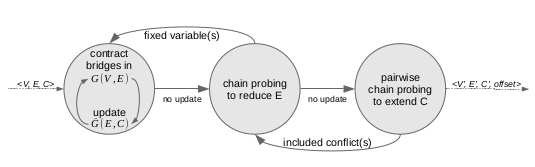
\includegraphics[width=0.9\textwidth]{img/peprocessing.png}
\end{figure}
    

\begin{block}{étapes}
\begin{enumerate}
    \item  Une contraction dans la première étape des arêtes pont(bridges).
    \item une suppression d'arête $e$ tel que $\delta_{ \hat{G}}(e) > 0 $, si la suppression de ses arêtes en conflits déconnecte le graphe, puis mise à jour de C.
    \item Choisir $e_{1},e_{2}$ tel que $\{e_{1},e_{2}\} \not\in C$ , si la suppression de leurs conflits déconnecte le graphe alors ajouter $\{e_{1},e_{2}\} \in C$ .
\end{enumerate}
   

\end{block}

\end{frame}
\begin{frame}{Algorithme de prétraitement}
\begin{block}{phase 01}

\end{block}

    
\end{frame}

\begin{frame}{Algorithme de prétraitement}
\begin{block}{Phase 02}
 \forall $ e_{i},e_{j}   \not\in C $, $\delta_{ \hat{G}}(e) > 0 $, ajouter \{$e_{i},e_{j}\} \in C$\quad SSI \quad G'=(V, E') est non connexe avec E'=E/$\{e_{i},e_{j}\}$
\end{block}

\textbf{Démonstration par l'absurde}
\newline
Supposant que $x_{e_{i}}=1$ \quad \textbf{$\Rightarrow $} \quad   $e_{j}=0$ car $\{e_{i},e_{j}\} \in S $; 
\newline Or $G/\{e_{j}\}$ non connexe.
\newline \textbf{contradiction} avec $X^*$ est un arbre.
\end{frame}
\begin{frame}{Algorithme de prétraitement}
\begin{block}{phase 03}
\forall $ e_{i},e_{j} \in E $\; Tq $\{e_{i},e_{j}\} \not\in C. $\newline
Soit $\chi(e_{i})$ et  $\chi(e_{j})$ l'ensemble des arêtes en conflit de $e_{i}$ et $e_{j}$ respectivement.
si G/$\chi(e_{i}) \cup \chi(e_{j})$ n'est pas connexe alors ajouter $\{e_{i},e_{i}\} \in S $
\end{block}
\textbf{Démonstration  par l'absurde}

    
\end{frame}

\section{Approche Branch and Cut}


\subsection{Formulation de programmation entière}
\begin{frame}{Approche Branch and Cut}
    \begin{block}{Formulation en programmation entiére}
    {\color{blue}  
        \begin{equation}
            \sum_{e \in E(S)} x_{e} \leq |S|-1 \qquad  \forall S \subset V, S \neq \phi 
        \end{equation}    
        
        \begin{equation}
             \sum_{e \in E} x_{e} = n-1
        \end{equation}
        
        \begin{equation}
            0\leq x_{e} \leq 1 \qquad  e \in E  
        \end{equation}
         
        \begin{equation}
            x_{e_{1}} + x_{e_{2}} \leq 1 \qquad  \forall{x_{e_{1}}, x_{e_{2}}} \in C  
        \end{equation}
         
        \begin{equation}
             \sum_{e \in U} x_{e} \leq \frac{|U|-1}{2}  \quad  \forall U \subset E \; \text{ incluant un odd-cycle dans }   \hat{G} 
        \end{equation}
    }
        \begin{equation}
             \sum_{e \in Q} x_{e} \leq 1  \quad  \forall Q \subset E \; \text{ une clique dans }   \hat{G} 
        \end{equation}
        \end{block}
\end{frame}

\begin{frame}{Approche Branch and Cut}
    \begin{block}{Article de F. Carrabs, R.Cerulli, R.Pentangelo, A.Raiconi}
        \begin{equation}
             \sum_{e_{i} \in \zeta}x_{e_{i}} \leq \zeta-1  \quad  \forall \zeta \subseteq E : \; \exists\{e_{k},e_{j}\}\subseteq \zeta \cap \chi(e_{c}), \; e_{c} \not\in \zeta
        \end{equation}
        
        \begin{equation}
             \sum_{e \in \delta(v)} x_{e} \geq 1  \quad  \forall v \subset V \; \text{ Pas de sommet isolé }  
        \end{equation}
    \end{block}
\end{frame}

\begin{frame}{Approche Branch and Cut}
    \begin{block}{Procédure de séparation}
        \begin{enumerate}
            \item Subtour elimination constraints
                \begin{itemize}
                    \item on construit un réseau orienté X; tel que la capacité d'un arc (i,j) correspond au poid de l'arête $X_{i,j}$ dans G.
                    \item on choisit arbitrairement un sommet r comme racine.
                    \item X satisfait SEC ssi on peut envoyer une unité de flux de r vers tous les sommet.
                    \item  si la valeur de toute coupe minimale est moins de 1, nous avons trouvé une enégalité violée.
                \end{itemize}
                
            \item Odd-cycle inequalities 
                \begin{itemize}
                    \item procédure de séparation exacte.
                \end{itemize}
        \end{enumerate}
    \end{block}
\end{frame}

%\subsection{Algorithme général}
%\input{files/metodologia.tex}

\subsection{Procédure de séparation}
%\input{files/metodologia.tex}



\section{Conclusion}
\begin{frame}{Conclusion}
\begin{itemize}
\item Approche exacte pour MSTCC
\item Agorithme de prétraitement
\item Formulation IP
\item Approche Branch and Cut
\end{itemize}
    
\end{frame}



\end{document}